\chapter{\IfLanguageName{dutch}{Stand van zaken}{State of the art}}
\label{ch:stand-van-zaken}

\section{Inleiding}
In dit hoofdstuk wordt een overzicht gegeven van de huidige stand van zaken rondom mobiele applicatieontwikkeling. De focus ligt daarbij op beveiliging, de keuze van platformen en cross-platform technologieën. Het doel is om de technologische context van dit project helder in kaart te brengen, zodat er een weloverwogen keuze kan worden gemaakt voor het meest geschikte ontwikkelplatform. Door recente ontwikkelingen en relevante literatuur te bespreken, leggen we een stevige basis voor de onderzoeksvragen en ontwerpbeslissingen die hierop volgen.

\section{Vergelijking van mobiele ontwikkelstrategieën}

Mobiele applicaties kunnen op uiteenlopende manieren worden ontwikkeld, afhankelijk van factoren zoals doelstellingen, budget, gewenste gebruikerservaring en technische vereisten. De keuze voor een specifieke ontwikkelstrategie is vaak bepalend voor het succes van een mobiele toepassing. Elke aanpak brengt namelijk eigen afwegingen met zich mee op het gebied van prestaties, onderhoud, ontwikkelsnelheid en compatibiliteit met verschillende platformen \autocite{Sharma2025}.\\

In deze sectie worden drie gangbare benaderingen uiteengezet: \textit{native development}, \textit{progressive web apps} (PWA’s) en \textit{cross-platform development}. Het doel is om een helder inzicht te geven in de principes van deze strategieën, zonder daarbij al in te gaan op specifieke tools of frameworks die komen later aan bod.\\

De bespreking en vergelijking van deze strategieën vindt plaats aan de hand van meerdere relevante criteria, waaronder prestaties, gebruikservaring, onderhoudsgemak, ontwikkelkosten en time-to-market. Deze analyse vormt de inhoudelijke basis voor het bepalen van de meest geschikte ontwikkelrichting binnen dit project.



\subsection{Native apps}
Een native app is een mobiele applicatie die specifiek is ontworpen voor een bepaald besturingssysteem of platform, zoals Android of iOS. Deze apps worden gebouwd met behulp van programmeertalen en ontwikkeltools die specifiek zijn voor dat platform. Voor Android zijn dat bijvoorbeeld Kotlin of Java, en voor iOS Swift of Objective-C. Native apps worden geïnstalleerd via de officiële appstores (Google Play of App Store) en draaien rechtstreeks op het besturingssysteem van het apparaat \autocite{Singh2024}.\\

Het grote voordeel van deze aanpak is dat native apps volledig kunnen profiteren van de functies van het besturingssysteem en de hardware van het apparaat. Denk hierbij aan toegang tot de camera, GPS, pushmeldingen, en een native gebruikersinterface. Volgens \textcite{Gillis2022} levert deze vorm van appontwikkeling de beste prestaties en de diepste integratie met het platform.\\

Een belangrijk voordeel is dat native apps een optimale gebruikerservaring bieden: ze voelen als een natuurlijk onderdeel van het platform, laden snel, tonen vloeiende animaties en volgen consistente interactiepatronen \autocite{Gillis2022}. Daartegenover staat dat deze aanpak vaak aparte ontwikkelteams per platform vereist, wat kan leiden tot hogere kosten en een langere time-to-market.

\subsection{Progressive Web Apps (PWA)}  
Progressive Web Apps zijn webapplicaties die zich gedragen als native apps. Ze maken gebruik van moderne webtechnologieën zoals HTML5, CSS3 en JavaScript, in combinatie met service workers en manifest-bestanden. PWA’s draaien in een browseromgeving, maar kunnen ook offline functioneren, pushnotificaties versturen en op het startscherm van een toestel worden geplaatst. PWA’s laden bij de eerste keer de volledige applicatie in en functioneren daarna vrijwel zelfstandig, zelfs bij slechte of afwezige internetverbindingen \autocite{Hendriksen2020}.\\

De belangrijkste voordelen van PWA’s zijn hun platformonafhankelijkheid en relatief lage ontwikkelkosten: één codebase is voldoende voor alle apparaten met een moderne browser. De functionaliteit is echter beperkter dan bij native apps, vooral wat betreft toegang tot hardware en beveiligde API’s.\\  

Een API (Application Programming Interface) is een software-interface die ervoor zorgt dat verschillende applicaties met elkaar kunnen communiceren. Je kunt het vergelijken met een ober in een restaurant: jij geeft een bestelling door, de ober neemt die bestelling mee naar de keuken (de server) en brengt het bereide gerecht terug naar jou. Op deze manier kunnen applicaties via API’s data opvragen en uitwisselen zonder dat zij direct toegang hebben tot elkaars systemen \autocite{Schoemaker2019}.\\  

Bij PWA’s worden API’s bijvoorbeeld gebruikt om informatie op te halen, zoals gebruikersdata, pushnotificaties te versturen of betalingen te verwerken. Pushnotificaties vormen een belangrijk communicatiemiddel tussen applicatie en gebruiker en krijgen daarom later in dit document een aparte bespreking (zie hoofdstuk \ref{sec:pushnotificaties}). Omdat iOS nog beperkingen kent op bepaalde API-functionaliteiten, werkt niet alle functionaliteit in een PWA op iPhones even volledig als op Android.\\  

De markt voor PWA’s groeit snel. In 2023 werd de wereldwijde marktwaarde geschat op 1,46 miljard USD, met een verwachte jaarlijkse groei van 31,1 procent tussen 2024 en 2030 \autocite{Research2024}. Deze groei wordt gedreven door factoren zoals de toenemende internetpenetratie en de vraag naar snelle, toegankelijke mobiele ervaringen. Grote bedrijven zoals Tinder, X (voorheen Twitter) en Forbes maken al gebruik van PWA-technologie. Figuur~\ref{fig:pwa_market} toont de verwachte marktgroei tot 2030.\\  


\begin{figure}[h]
    \centering
    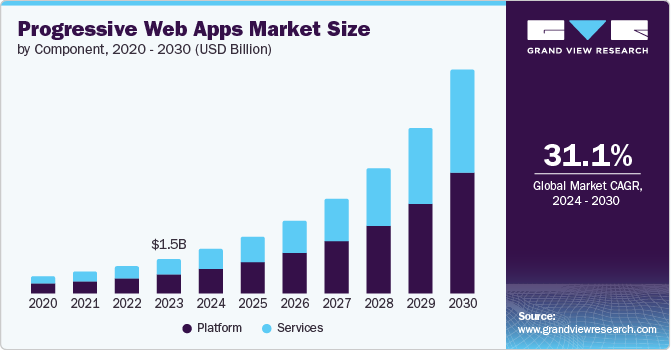
\includegraphics[width=0.75\textwidth]{pwa-market.png}
    \caption{Wereldwijde marktgroei van Progressive Web Apps (USD miljard), 2020–2030. Bron: Grand View Research, 2025. \autocite{Research2024}}
    \label{fig:pwa_market}
\end{figure}

\subsection{Cross-platform frameworks}
Cross-platform frameworks zoals Flutter, React Native en .NET MAUI vormen een middenweg tussen de prestaties van native apps en de snelle ontwikkeltijd van PWA’s. Ze maken het mogelijk om met één gedeelde codebase applicaties te ontwikkelen voor meerdere platformen, wat de ontwikkeltijd verkort en onderhoudskosten verlaagt \autocite{Kuppan2024}.\\

Flutter en React Native gebruiken eigen rendering-engines of native componenten voor de gebruikersinterface, terwijl .NET MAUI direct platform-native UI-elementen aanspreekt via .NET-technologie. Uit onderzoek blijkt dat Flutter uitblinkt in vloeiende animaties en UI-prestaties, terwijl .NET MAUI sterk is in integratie met Microsoft-omgevingen \autocite{Gajjam2025}. Toch blijven cross-platform apps soms iets achter bij native apps, vooral bij grafisch intensieve of rekenintensieve toepassingen.

\begin{table}[h]
    \centering
    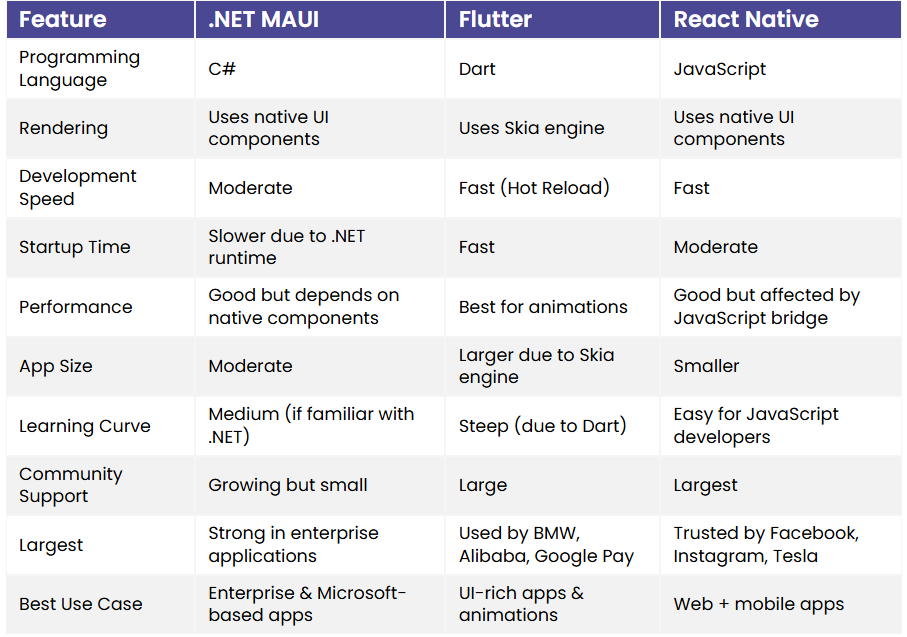
\includegraphics[width=0.8\textwidth]{comparison1.png}
    \caption[Integratie]{Vergelijking van .NET MAUI, Flutter en React Native op basis van geschiktheid voor enterprise-omgevingen \autocite{Gajjam2025}}
    \label{fig:vergelijking}
\end{table}

\begin{table}[h]
    \centering
    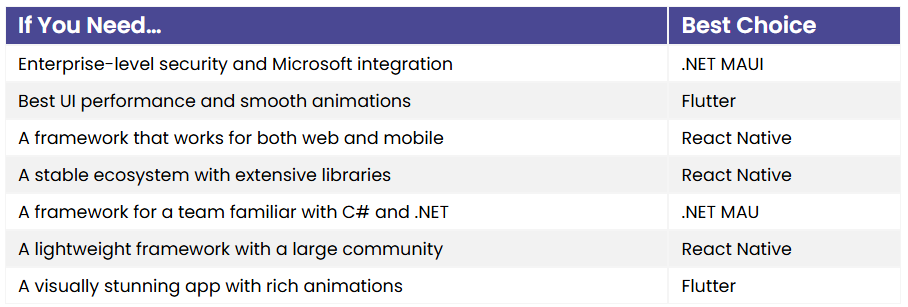
\includegraphics[width=0.8\textwidth]{comparison2.png}
    \caption[Frameworkkeuze]{Overzicht van aanbevolen cross-platform frameworks (Flutter, React Native en .NET MAUI) op basis van specifieke projectvereisten \autocite{Gajjam2025}}
    \label{tab:frameworkkeuze}
\end{table}

\subsection{Samenvatting en aanbevelingen}
Welke mobiele ontwikkelstrategie het beste past, hangt af van de context, de doelstellingen en de technische randvoorwaarden van het project. Uit voorgaand onderzoek blijkt dat native apps bijzonder geschikt zijn voor toepassingen waarbij maximale prestaties en een hoogwaardige gebruikerservaring cruciaal zijn, bijvoorbeeld bij games of apps met intensieve interactie \autocite{Singh2024, Gillis2022}. Deze aanpak zorgt voor optimale integratie met het besturingssysteem en directe hardwaretoegang, maar vergt vaak aparte teams per platform, wat hogere kosten en een langere ontwikkeltijd tot gevolg heeft.\\

Progressive Web Apps bieden een kosteneffectieve, platformonafhankelijke oplossing, met één codebase voor alle moderne browsers \autocite{Hendriksen2020, Research2024}. Ze zijn geschikt voor eenvoudige of informatieve apps zonder complexe functies. De functionaliteit is echter beperkter, vooral wat betreft hardwaretoegang en beveiligde API’s. Ook is de ondersteuning voor bepaalde functies, zoals pushnotificaties op iOS, nog beperkt \autocite{Schoemaker2019}.\\

Cross-platform frameworks als Flutter, React Native en .NET MAUI vormen een aantrekkelijk compromis: met één gedeelde codebase kunnen apps voor meerdere platformen worden ontwikkeld, wat de ontwikkeltijd verkort en het onderhoud vereenvoudigt \autocite{Kuppan2024}. Flutter onderscheidt zich door uitstekende UI-prestaties en animaties, terwijl .NET MAUI een goede keuze is voor organisaties die diep in het Microsoft-ecosysteem zitten, mede dankzij de integratie met Visual Studio en Azure \autocite{Gajjam2025}.\\

Figuur~\ref{fig:vergelijking} toont een overzicht van de voor- en nadelen van deze strategieën. De beste keuze hangt af van het doel van de app, de gewenste gebruikerservaring en de beschikbare middelen. Zo is .NET MAUI vaak de beste optie in enterprise-omgevingen waar stabiliteit, veiligheid en integratie centraal staan, terwijl native ontwikkeling of PWA’s beter kunnen passen bij specifieke projectdoelen en budgetten.\\

Kortom, door zorgvuldig af te wegen tussen prestaties, ontwikkeltijd, functionaliteit en de organisatorische context, kan een projectteam een mobiele ontwikkelstrategie kiezen die zowel aan technische als zakelijke eisen voldoet.\\


\section{Vergelijking van Cross-Platform Frameworks}

\subsection{Wat is een UI-framework?}
Een UI-framework (User Interface framework) is een verzameling vooraf gebouwde, herbruikbare componenten, stijlen en tools die het ontwikkelen van gebruikersinterfaces vereenvoudigt en versnelt. Denk hierbij aan standaardcomponenten zoals knoppen, formulieren en navigatiebalken, die consequent zijn vormgegeven en functioneren. UI-frameworks zorgen voor ontwerpconsistentie binnen een applicatie, versnellen het ontwikkelproces en zijn vaak responsief ontworpen, zodat applicaties goed werken op verschillende apparaten en schermformaten \autocite{Coditation2023}.\\

Het gebruik van een UI-framework brengt voordelen met zich mee, zoals snellere ontwikkeling, een uniforme gebruikerservaring en toegang tot een actieve community voor ondersteuning. Tegelijkertijd kunnen sommige frameworks ook beperkingen opleveren, bijvoorbeeld qua performance of aanpasbaarheid, afhankelijk van de projectbehoeften.\\

\subsection{Flutter}
Flutter is een open-source UI-framework van Google, gebaseerd op de programmeertaal Dart. Het staat bekend om hoge prestaties, vloeiende animaties en een uitgebreide set widgets, die dienen als de visuele en interactieve onderdelen van een app. Een widget kan bijvoorbeeld een knop, een tekstveld of een menu zijn, en vormt steeds een klein stukje van de gebruikersinterface. Door deze widgets slim te combineren, kunnen ontwikkelaars op een eenvoudige manier professionele en consistente apps bouwen. Daarnaast biedt Flutter ondersteuning voor plug-ins, die extra mogelijkheden toevoegen aan een app zonder dat deze volledig zelf ontwikkeld hoeven te worden. Denk hierbij aan functies zoals het openen van de camera, het bepalen van de locatie of het opslaan van gegevens op het toestel. Flutter ondersteunt iOS, Android, web en desktop, en profiteert van een groeiende community met een grote hoeveelheid beschikbare widgets en plug-ins \autocite{Gajjam2025}.\\

Een onderscheidend kenmerk is \emph{hot reload}, dit betekent dat ontwikkelaars realtime wijzigingen kunnen doorvoeren. Wat de ontwikkelsnelheid sterk verhoogt. Flutter ondersteunt zowel Material Design als Cupertino-stijl en maakt gebruik van de Skia-renderengine voor consistente prestaties \autocite{Rodriguez2025}.\\

In 2023 gebruikte 46\% van ontwikkelaars wereldwijd Flutter, waarmee het het populairste cross-platform framework is. Grote merken zoals Google Ads, BMW en Alibaba vertrouwen op Flutter, wat de kracht van één codebase en besparingen in tijd en kosten benadrukt. Figuur~\ref{fig:flutter} toont een overzicht van het gebruik van verschillende frameworks.\\

Een beperking is de matige integratie met enterprise-systemen en Microsoft-\\technologieën, wat voor organisaties die sterk op het Microsoft-ecosysteem\\ steunen een nadeel kan zijn.

\subsection{React Native}
React Native, ontwikkeld door Meta, maakt het mogelijk mobiele apps te bouwen met JavaScript en React. Het biedt een goede balans tussen snelheid, performance en schaalbaarheid, zeker in combinatie met het Expo-platform dat native build-omgevingen vereenvoudigt \autocite{Ivanov2025}.\\

Met één codebase voor iOS en Android worden ontwikkeltijden verkort en kosten gedrukt, wat vooral aantrekkelijk is voor kleine teams. Expo voegt hier hot reloading en een managed workflow aan toe, plus de Expo Go-app voor directe testing op fysieke apparaten \autocite{Ivanov2025}.\\

Een managed workflow betekent dat veel technische details automatisch voor je worden geregeld. Hierdoor kunnen ontwikkelaars zich vooral richten op het schrijven van de app zelf, zonder zich zorgen te maken over ingewikkelde instellingen of installatieproblemen. Dit maakt het ontwikkelen makkelijker en sneller, vooral voor teams die niet veel tijd of ervaring hebben met het bouwen van apps.\\

React Native maakt het mogelijk om apps te bouwen die aanvoelen alsof ze speciaal voor een bepaald toestel zijn gemaakt. Dit gebeurt doordat de technologie contact maakt met functies van het toestel zelf, zoals de camera of het touchscreen. Bewegingen en overgangen in de app, zoals het schuiven van een menu of het openen van een scherm, verlopen meestal soepel dankzij speciale hulpmiddelen voor animaties \autocite{Ivanov2025}. Dankzij zogenaamde Over-the-Air updates, waarbij de aanpassingen draadloos via het internet naar de app worden gestuurd, kunnen kleine veranderingen of foutoplossingen snel bij gebruikers terechtkomen zonder dat de app opnieuw via de appwinkel hoeft te worden gedownload.\\

Echter, voor complexe platform-specifieke functies is vaak native code nodig, wat extra onderhoud vergt. De integratie met Microsoft-technologieën is beperkt, waardoor .NET MAUI vaak de voorkeur heeft in enterprise-omgevingen met Azure en .NET-backends \autocite{Longe2025}.

\subsection{.NET MAUI}
.NET MAUI, de opvolger van Xamarin, is Microsofts nieuwste cross-platform framework. Het stelt ontwikkelaars in staat met één codebase apps te bouwen voor iOS, Android, Windows en macOS, wat kosten en onderhoud reduceert \autocite{Sheth2024}.\\

De diepe integratie met het Microsoft-ecosysteem (zoals Visual Studio, Azure en .NET Core) zorgt ervoor dat ontwikkelaars in één vertrouwde werkomgeving kunnen werken, met dezelfde hulpmiddelen en standaarden voor alle onderdelen van het project \autocite{Sheth2024}. Dit betekent dat programmeurs, testers en ontwerpers eenvoudiger kunnen samenwerken, omdat iedereen met dezelfde set software werkt en over dezelfde documentatie beschikt. Visual Studio ondersteunt hierbij handige functies als Hot Reload en Live Preview, waarmee aanpassingen direct zichtbaar zijn zonder de applicatie helemaal opnieuw te hoeven opstarten, wat de ontwikkelcyclus aanzienlijk versnelt.\\

Dankzij een enkele projectstructuur maakt .NET MAUI het makkelijker om apps voor verschillende apparaten te ontwikkelen. De gebruiksvensters en knoppen passen zich automatisch aan het besturingssysteem aan \autocite{Sheth2024}. Hierdoor krijgt de gebruiker overal een gelijkwaardige ervaring, terwijl het uiterlijk van het merk behouden blijft.\\

Performance is sterk dankzij efficiënt geheugenbeheer, snelle opstarttijden en directe toegang tot native API’s. Platform-specifieke extensies zijn mogelijk via custom handlers zonder de gedeelde codebasis te verlaten.\\

Voor organisaties die zwaar investeren in Microsoft-technologieën biedt .NET MAUI een strategisch voordeel door naadloze integratie met ASP.NET Core en Azure App Services \autocite{Klesman2023}.

\begin{figure}[h]
    \centering
    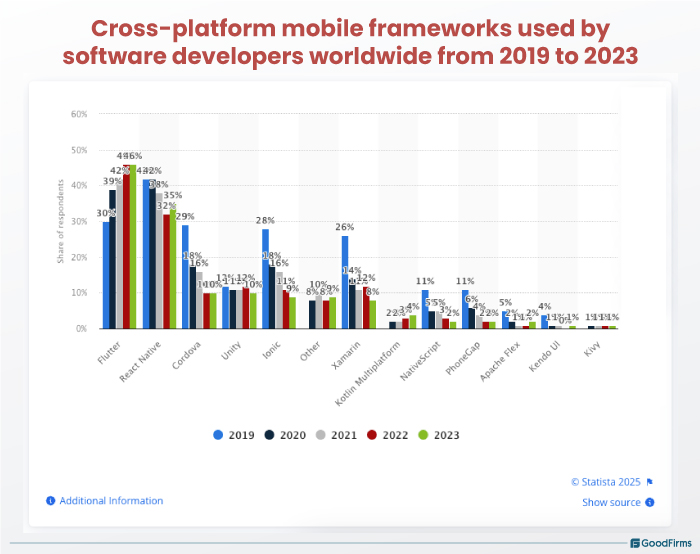
\includegraphics[width=0.75\textwidth]{flutter.jpg}
    \caption{Gebruik van cross-platform frameworks onder ontwikkelaars in 2023. Bron: Statista \autocite{Rodriguez2025}}
    \label{fig:flutter}
\end{figure}

\subsection{Technologische Continuïteit}
Gezien ATS reeds intensief werkt met het .NET-ecosysteem (C#, ASP.NET Core, Azure), sluit .NET MAUI optimaal aan. Dit vermindert de leercurve, vereenvoudigt integratie en onderhoud, terwijl Flutter en React Native aanvullende kennis en inspanning vereisen \autocite{Longe2025}.

\subsection{Samenvatting en Aanbeveling}
Flutter, React Native en .NET MAUI bieden elk unieke voordelen. Flutter is ideaal voor visueel rijke apps en snelle ontwikkeling, React Native voor brede platformondersteuning en een grote community, terwijl .NET MAUI uitblinkt in integratie met Microsoft-technologie en enterprise-functionaliteit.\\


ATS heeft een voorkeur voor Microsoft-technologie, .NET MAUI zorgt ervoor dat er wordt voldaan aan de enterprise-eisen. Men kan technologische continuïteit garanderen door het hergebruiken van eerdere kennis en het behouden van een consistente gebruikservaring. 

\section{Vergelijking van software-architecturen voor mobiele applicaties}

Softwarearchitectuur vormt de fundamentele structuur van een softwaretoepassing, waarbij de verschillende componenten, hun onderlinge relaties en interacties worden gedefinieerd. In de context van mobiele applicaties is een goede softwarearchitectuur cruciaal om de complexiteit van de app te beheersen, zeker omdat deze applicaties vaak worden ontwikkeld voor diverse apparaten met uiteenlopende specificaties en korte releasetijden \autocite{Dobrean2019}. \\

Een geschikte architectuur helpt ontwikkelaars om het systeem onderhoudbaar, uitbreidbaar en testbaar te houden. Daarnaast maakt het mogelijk om afhankelijkheden tussen componenten te beheersen en bevordert het hergebruik van code. Zoals \textcite{Dobrean2019} benadrukt, voorkomt een doordachte architectuur het ontstaan van grote, moeilijk te onderhouden klassen, en helpt het ontwikkelteam sneller nieuwe functies toe te voegen zonder bestaande functionaliteit te breken.\\

In deze sectie worden diverse architectuurmodellen besproken die relevant zijn voor de ontwikkeling van mobiele applicaties. Per model worden de kernprincipes, voordelen, nadelen en de aansluiting bij projectvereisten toegelicht. Daarnaast wordt ingegaan op de implementatie binnen het Android-platform, gebaseerd op het onderzoek van \textcite{Lou2016}.\\

\subsection{Model-View-Controller (MVC)}
Het Model-View-Controller (MVC) patroon, geïntroduceerd in Smalltalk-80 en grondslag voor moderne architecturen, verdeelt de applicatie in drie componenten \autocite{Lou2016}:  
\begin{itemize}
	\item Model: Beheert de data en businesslogica, al dan niet via externe bronnen.  
	\item View: De gebruikersinterface die de data visualiseert.  
	\item Controller: Ontvangt gebruikersinput, past het model aan en communiceert veranderingen aan de view.  
\end{itemize}

Zoals \textcite{Lou2016} beschrijven, is de relatie tussen View en Controller meestal één-op-één en sterk gekoppeld. De View is het gedeelte van de app dat de gebruiker ziet en waarmee hij of zij interactie heeft, zoals knoppen, tekstvelden of afbeeldingen. De Controller is het onderdeel dat deze interacties afhandelt en bepaalt wat er gebeurt wanneer een gebruiker iets doet, bijvoorbeeld een knop indrukt. De modelcomponent bevat de onderliggende gegevens en logica van de app en kan aan meerdere View-Controller-paren gekoppeld zijn, wat synchronisatie-uitdagingen oplevert wanneer de gegevens veranderen.\\

MVC (Model-View-Controller) is standaard de basisarchitectuur voor native Android-apps, hoewel de scheiding tussen View en Controller in de praktijk vaak minder strikt is. In Android wordt de Controller meestal vertegenwoordigd door een Activity of Fragment, terwijl de View bestaat uit XML-layoutbestanden (die beschrijven hoe de interface eruitziet, XML staat voor eXtensible Markup Language) en UI-widgets zoals knoppen, tekstvelden en lijsten.\\

\subsection{Model-View-Presenter (MVP)}
MVP is een evolutie van MVC die een duidelijkere scheiding van verantwoordelijkheden beoogt \autocite{Lou2016}.  
Belangrijke componenten zijn:  
\begin{itemize}
	\item Model: Zoals in MVC, beheert data en businesslogica.  
	\item View: Toont data en interface, zonder logica.  
	\item Presenter: Beheert alle UI-logica en interacties tussen Model en View.  
\end{itemize}

In tegenstelling tot MVC start de interactiestroom bij de \View, oftewel het scherm dat de gebruiker ziet. De View geeft gebruikersinput, zoals klikken op knoppen of invullen van velden, door aan de Presenter. De Presenter verwerkt deze input, werkt het Model bij indien nodig, en past daarna de View aan \autocite{Lou2016}.\\

Door dit patroon wordt de koppeling tussen View en Model kleiner, waardoor unit testing eenvoudiger wordt. Unit testing betekent dat kleine stukjes code, zoals functies of klassen, afzonderlijk getest worden om te controleren of ze correct werken.\\

Bij de Passive View-variant wordt de View zo “\textit{dumb}” mogelijk gemaakt. Dit betekent dat de View zelf zo min mogelijk logica bevat. Het scherm toont alleen informatie en stuurt input door. Alle beslissingen en verwerking gebeuren in de Presenter, waardoor de code overzichtelijk blijft en eenvoudiger te testen is \textcite{Lou2016}.\\


\subsection{Model-View-ViewModel (MVVM)}
MVVM is speciaal ontworpen voor moderne UI-frameworks en stelt de View in staat om door middel van databinding direct gekoppeld te zijn aan de ViewModel \autocite{Lou2016}.  
\begin{itemize}
	\item Model: Beheert de data en businesslogica.  
	\item View: De UI, vaak ontworpen door een designer, die databinding ondersteunt.  
	\item ViewModel: Houdt de status van de View bij, beheert UI-logica en exposeert data en commando’s via properties.  
\end{itemize}

Door databinding kan de View automatisch reageren op veranderingen in de ViewModel zonder expliciete code. Dit vereenvoudigt de UI-ontwikkeling en onderhoudbaarheid aanzienlijk. In Android wordt MVVM vaak geïmplementeerd met behulp van de databinding-library, waarbij XML-layouts rechtstreeks gebonden worden aan ViewModel-gegevens en -methoden.

\subsection{Conclusie}
Hoewel MVC de basis vormt, bieden MVP en MVVM een betere scheiding van verantwoordelijkheden en testbaarheid. MVVM onderscheidt zich door zijn databinding-ondersteuning, die naadloze synchronisatie tussen View en ViewModel mogelijk maakt, hetgeen binnen \texttt{.NET MAUI} en moderne Android-ontwikkeling sterk wordt aanbevolen. De keuze voor een architectuur hangt af van het project, de benodigde flexibiliteit en het framework waarmee gewerkt wordt \autocite{Lou2016}.


\section{Moderne Authenticatie en Beveiligingspraktijken}

\subsection{Vergelijking van moderne authenticatiemethoden}

Mobiele authenticatie is belangrijk om te zorgen dat alleen geautoriseerde gebruikers toegang krijgen tot gevoelige gegevens en diensten op hun mobiele apparaten. Er bestaan verschillende methoden, elk met eigen voor- en nadelen.\\

Een veelgebruikte methode is sessiegebaseerde authenticatie. Hierbij houdt de server bij wie er is ingelogd door een tijdelijke sessie aan te maken. Dit werkt goed, maar kan problemen geven wanneer er veel gebruikers zijn, omdat de server al die sessies moet beheren \autocite{Gao2023}.\\

OAuth2 is een systeem dat vaak gebruikt wordt om gebruikers via één account toegang te geven tot meerdere diensten (bijvoorbeeld inloggen met je Google-account op andere websites). Dit heet ook wel federatieve toegang. OAuth2 is krachtig maar relatief ingewikkeld, en daarom soms minder geschikt voor eenvoudige apps die alleen intern gebruikt worden \autocite{Gao2023}.\\

JSON Web Tokens (JWT) zijn een lichtere en flexibelere manier om authenticatie te regelen. Hierbij worden gegevens over de gebruiker opgeslagen in een digitaal token dat de gebruiker meebrengt bij elk verzoek. Omdat de server deze tokens niet hoeft bij te houden, werkt het sneller en is het makkelijker schaalbaar. Dit maakt JWT populair in moderne systemen zoals cloudomgevingen en microservices \autocite{Gao2023}.\\

Naast deze methoden voor het vaststellen wie toegang krijgt, zijn er verschillende manieren om de identiteit van de gebruiker te controleren. De meest traditionele methode is het gebruik van wachtwoorden, waarbij gebruikers een geheime code invoeren. Hoewel dit veel voorkomt, zijn wachtwoorden kwetsbaar voor aanvallen zoals raden of diefstal \autocite{Zukarnain2022}.\\

Een veiliger alternatief is dynamische wachtwoorden, bijvoorbeeld via een sms-code. Hierbij krijgt de gebruiker een eenmalige code op zijn telefoon, die hij moet invoeren. Dit vermindert het risico op misbruik, maar sms-berichten kunnen onderschept worden \autocite{Zukarnain2022}.\\

Biometrische authenticatie maakt gebruik van unieke lichaamskenmerken zoals een vingerafdruk of gezichtsherkenning. Dit is handig omdat het snel en gebruiksvriendelijk is, en deze kenmerken moeilijk te vervalsen zijn. Toch is het een risico als biometrische data gelekt worden, want die kunnen niet veranderd worden zoals een wachtwoord \autocite{Zukarnain2022}.\\

Er zijn ook vernieuwende methoden zoals trajectgebaseerde authenticatie, waarbij het systeem kijkt naar de gebruikelijke reisroutes van een persoon om te controleren of het echt de juiste gebruiker is. Dit werkt minder goed voor mensen die vaak reizen of van locatie wisselen \autocite{Zukarnain2022}.\\

Zoals \textcite{Zukarnain2022} benadrukt, is het belangrijk dat verschillende partijen, zoals mobiele netwerkproviders (operators), tussenpersonen (aggregators) en app-aanbieders (merchants), samenwerken. Elke partij hanteert eigen beveiligingsmethodes, wat de situatie complex maakt. Het samenbrengen van al deze methoden op één platform kan de veiligheid verhogen en het beheer vereenvoudigen.\\

Kortom, mobiele authenticatie is een ingewikkeld vakgebied waarbij veiligheid, gebruiksgemak en snelheid goed in balans moeten worden gehouden \autocite{Zukarnain2022, Gao2023}.\\


\subsection{Overwegingen bij wachtwoordbeveiliging}
Het veilig opslaan van wachtwoorden is essentieel om te voorkomen dat kwaadwillenden toegang krijgen tot accounts. Hiervoor worden technieken gebruikt zoals hashing en salting. Bij hashing wordt het wachtwoord omgezet in een vaste reeks tekens, een zogenaamde hash, die niet eenvoudig terug te herleiden is naar het oorspronkelijke wachtwoord \autocite{Gupta2022}.\\

Omdat dezelfde wachtwoorden zonder extra bescherming altijd dezelfde hash opleveren, voegt men een unieke, willekeurige waarde toe: de salt. Deze salt zorgt ervoor dat zelfs als twee gebruikers hetzelfde wachtwoord kiezen, de hashes toch verschillend zijn. Dit voorkomt dat aanvallers met vooraf berekende lijsten, zoals rainbow tables, gemakkelijk wachtwoorden kunnen kraken \autocite{Arias2025}.\\

Rainbow tables zijn vooraf berekende tabellen die worden gebruikt om hashes terug te vertalen naar hun oorspronkelijke wachtwoorden. In plaats van voor elke poging opnieuw alle hashingoperaties uit te voeren, kan een aanvaller de tabel raadplegen om snel overeenkomende wachtwoorden te vinden (zie Figuur~\ref{fig:rainbowtable}). Zoals \textcite{ViniciusFulberGarcia2024} uitleggen, bevatten deze tabellen combinaties van oorspronkelijke invoer (plaintext) en de bijbehorende hashcodes, waardoor het eenvoudiger wordt om gestolen hashlijsten te kraken.\\

\begin{figure}[h]
	\centering
	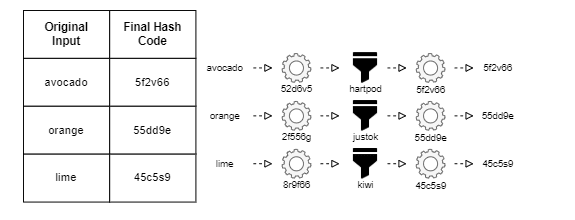
\includegraphics[width=0.75\textwidth]{rainbowtable.png}
	\caption{Voorbeeld van een simpele rainbow table \autocite{ViniciusFulberGarcia2024}}
	\label{fig:rainbowtable}
\end{figure}

Rainbow table-aanvallen beginnen meestal met het bemachtigen van een lijst van hashes, bijvoorbeeld via een kwetsbare database of phishingtechnieken. Vervolgens vergelijkt de aanvaller de hashes met de rainbow table om matches te vinden en zo de originele wachtwoorden te achterhalen. Salting, waarbij een unieke, willekeurige waarde aan het wachtwoord wordt toegevoegd voordat het gehasht wordt, maakt deze aanvallen aanzienlijk moeilijker \textcite{Arias2025}. Andere maatregelen, zoals het gebruik van sterke, unieke wachtwoorden en moderne hashing-algoritmes zoals bcrypt en PBKDF2, vergroten de weerstand tegen dit type aanval.\\

Voor het hashen van wachtwoorden worden moderne algoritmes zoals bcrypt en PBKDF2 aanbevolen. Deze algoritmes zijn ontworpen om extra rekentijd te vereisen, waardoor brute-force aanvallen—waarbij een aanvaller vele combinaties probeert—veel moeilijker en tijdrovender worden \autocite{Gupta2022}.\\

Verouderde algoritmes zoals MD5 en SHA1 worden afgeraden omdat ze kwetsbaar zijn en te snel werken, wat het makkelijker maakt om hashes te kraken \autocite{ReesCarter2024}.

\subsection{Beveiligde Login-interfaces}
Een veilige loginpagina is essentieel om gebruikersaccounts te beschermen, maar moet ook makkelijk in gebruik blijven. Een veelvoorkomend veiligheidsrisico is credential stuffing. Dit is een aanval waarbij criminelen lijsten met eerder gestolen gebruikersnamen en wachtwoorden gebruiken om in te loggen op andere websites of diensten. Omdat veel mensen dezelfde inloggegevens hergebruiken, kunnen deze aanvallen grote schade veroorzaken \autocite{Chinnasamy2025}.\\

Bij credential stuffing zetten aanvallers geautomatiseerde programma’s in die massaal proberen in te loggen met deze gestolen gegevens. Ze gebruiken verschillende IP-adressen, dat wil zeggen unieke nummers die elk apparaat op het internet identificeren, om detectie te ontwijken en vinden zo snel accounts die ze kunnen misbruiken. Om dit te voorkomen, is het belangrijk om mislukte inlogpogingen te beperken en gebruikers te dwingen sterke, unieke wachtwoorden te kiezen \autocite{Chinnasamy2025}.\\

Tweefactorauthenticatie (2FA) biedt een extra beveiligingslaag die het risico op ongeautoriseerde toegang sterk vermindert. Naast het invoeren van een gebruikersnaam en wachtwoord vraagt 2FA om een tweede bevestiging, zoals een eenmalige code (OTP) die bijvoorbeeld via sms of een speciale app op je telefoon wordt ontvangen. Pas als beide stappen correct zijn doorlopen, krijgt de gebruiker toegang tot het account \autocite{Jurisons2024}.\\

Deze tweede factor kan verschillende vormen aannemen: iets wat je weet (zoals een wachtwoord), iets wat je hebt (zoals een smartphone of token), of iets wat je bent (zoals een vingerafdruk). Door verschillende soorten factoren te combineren, wordt het veel moeilijker voor aanvallers om in te breken, zelfs als ze je wachtwoord kennen.\\

2FA heeft een balans tussen gebruiksgemak en veiligheid. Het is relatief betaalbaar, snel in te zetten, en doordat veel mensen al een mobiele telefoon bezitten, eenvoudig toe te passen. Natuurlijk kost het inloggen met 2FA iets meer tijd en moeite dan alleen een wachtwoord, en soms kan het tijdkosten doordat men moet wachten op een sms-code, maar de extra veiligheid compenseert deze voorgaande issues. \autocite{Jurisons2024}.\\

Toch is geen enkel systeem perfect: zeer geavanceerde aanvallers kunnen soms ook 2FA omzeilen. Phishing is bijvoorbeeld een techniek waarbij iemand misleid wordt om zijn inloggegevens vrijwillig te delen via nepwebsites of valse e-mails, terwijl malware kwaadaardige software is die ongemerkt toegang tot een apparaat kan geven. Daarom blijft het belangrijk om ook andere maatregelen te nemen, zoals het monitoren van verdachte loginpogingen, het gebruik van CAPTCHA’s. CAPTCHA's zijn kleine tests om te controleren of een gebruiker echt een mens is en geen geautomatiseerde bot—om bots te blokkeren, en het regelmatig updaten van beveiligingsprotocollen \autocite{Chinnasamy2025}.\\

Kortom, door sterke wachtwoorden te combineren met limieten op inlogpogingen en tweefactorauthenticatie kunnen organisaties hun loginpagina’s veel veiliger maken, terwijl ze gebruikers niet onnodig hinderen.\\

\subsection{Samenvattende overwegingen}
Moderne beveiliging vereist balans tussen schaalbaarheid, gebruiksgemak en veiligheid. JWT biedt een efficiënte, schaalbare aanpak in moderne architecturen, terwijl robuuste hashing en salting wachtwoordbeveiliging versterken. De gebruikersinterface moet beveiliging en gebruiksgemak combineren, bijvoorbeeld via 2FA en inlogpogingenlimiet. Deze overwegingen leiden tot een toekomstbestendige beveiligingsstrategie \autocite{Gao2023, Gupta2022, Arias2025, ReesCarter2024, Chinnasamy2025, Jurisons2024}.

\section{Beveiliging en Beheer van Pushnotificaties}
\label{sec:pushnotificaties}

\subsection{Onderzoek naar Technische Implementatieopties}
Volgens \textcite{Wohllebe2021} zijn pushnotificaties een krachtig middel om gebruikers snel te informeren, bijvoorbeeld over de status van zonnepanelen of slimme meters. Deze meldingen verschijnen direct op het scherm van je smartphone en zorgen ervoor dat je meteen op de hoogte bent van belangrijke updates.\\

Ontwikkelaars gebruiken hiervoor vaak speciale diensten die per platform verschillen. Voor Apple-toestellen is dat de Apple Push Notification Service (APNs) en voor Android-apparaten Firebase Cloud Messaging (FCM). Deze diensten zijn betrouwbaar en goed geïntegreerd in het systeem, waardoor ze vaak de beste keuze zijn voor toepassingen waarbij betrouwbaarheid belangrijk is \autocite{Wohllebe2021}.\\

Er bestaan ook diensten die voor meerdere platforms tegelijk werken, zoals OneSignal. Deze bieden extra functies en maken het beheer eenvoudiger, maar zorgen ook voor extra complexiteit en afhankelijkheid van een externe partij. Sommige bedrijven kiezen ervoor om zelf een systeem te bouwen. Hierbij worden bijvoorbeeld WebSockets gebruikt, waarmee apparaten en servers continu met elkaar verbonden blijven zodat berichten direct kunnen worden uitgewisseld, of MQTT (Message Queuing Telemetry Transport), een protocol dat efficiënt kleine berichten laat versturen tussen apparaten, zoals sensoren of apps. Zelf zo'n systeem opzetten is echter ingewikkelder en minder goed schaalbaar \textcite{Wohllebe2021}.\\

Hoe een pushnotificatie eruitziet, beïnvloedt de kans dat mensen erop reageren. Onderzoek laat zien dat een duidelijke titel in de melding het aantal gebruikers dat de app opent verhoogt. Extra elementen zoals plaatjes of knoppen blijken daarentegen niet significant bij te dragen aan meer interactie \autocite{Wohllebe2021}.\\

Pushnotificaties werken als een prikkel die de gebruiker aanzet tot actie, bijvoorbeeld het openen van een app. Of iemand hierop reageert, hangt af van hoe relevant en interessant de melding is. Relevante en persoonlijke informatie wordt vaker gewaardeerd en zorgt voor meer betrokkenheid. Tegelijkertijd kan een zekere mate van nieuwsgierigheid, bijvoorbeeld door het weglaten van details, ook de interactie stimuleren \autocite{Wohllebe2021}.\\

Het is wel belangrijk dat pushnotificaties niet te vaak worden verstuurd. Te veel meldingen kunnen als storend worden ervaren en leiden tot frustratie, waardoor gebruikers de meldingen kunnen uitschakelen. Daarom is het essentieel dat de berichten altijd nuttig en relevant zijn, zodat ze als waardevol worden gezien en niet als hinderlijk \autocite{Wohllebe2021}.\\

\subsection{Beheer en Verificatie van Tokens}
Om pushberichten op de juiste apparaten te bezorgen, wordt bij installatie van een app een uniek identificatienummer toegekend aan elk toestel, een zogenaamd push-token \autocite{pushwoosh2025}. Dit token is als het ware het adres waar meldingen naartoe worden gestuurd.\\

Toch kan zo’n token veranderen, bijvoorbeeld wanneer iemand de app verwijdert en opnieuw installeert, of bij een update van het besturingssysteem. Daarom is het belangrijk om regelmatig te controleren of het token nog klopt. Sommige apps doen dit automatisch bij het opstarten, zodat ze altijd met het juiste token werken. Dat is handig, maar zorgt ook voor iets meer internetverkeer.\\

Een andere mogelijkheid is om pas iets te doen als er een foutmelding komt bijvoorbeeld wanneer een pushbericht niet aankomt omdat het token ongeldig is. Dat is zuiniger qua netwerkverkeer, maar het kan wel betekenen dat iemand tijdelijk geen meldingen ontvangt totdat het probleem is ontdekt \autocite{pushwoosh2025}.\\

Volgens \textcite{pushwoosh2025} kiezen veel ontwikkelaars voor een combinatie van strategieën: ze vernieuwen het token bij het opstarten van de app, controleren periodiek of het nog klopt, en reageren als er iets misgaat. Deze aanpak zorgt ervoor dat meldingen betrouwbaar blijven aankomen, zonder dat er onnodig veel communicatie met de server nodig is.\\

\subsection{Gebruiksvormen van Pushnotificaties}

Pushnotificaties kunnen op verschillende manieren worden verstuurd, afhankelijk van wie je wil bereiken. Binnen Firebase Cloud Messaging (FCM) onderscheiden we drie gangbare methodes: multicast, device groups en topics. Elke methode heeft zijn eigen voordelen en is geschikt voor een specifiek gebruiksscenario.\\

\textbf{Multicast – meerdere toestellen tegelijk benaderen.}\\
Multicast is een methode waarbij één pushnotificatie tegelijk naar meerdere apparaten wordt gestuurd. Dit gebeurt via een lijst van apparaat-tokens, waarbij elk token een specifiek toestel vertegenwoordigt. Deze methode is vooral handig bij algemene meldingen die voor veel gebruikers tegelijk bedoeld zijn, zoals een storing of onderhoudsbericht. Firebase Cloud Messaging (FCM) ondersteunt tot 500 apparaten per multicast-verzoek.\\

In meer geavanceerde toepassingen, zoals bij locatiegebaseerde noodmeldingen, kan multicast ook slimmer worden ingezet. In plaats van een melding naar alle gebruikers te sturen, kan eerst bepaald worden welke gebruikers zich in een bepaald gebied bevinden — bijvoorbeeld bij een gaslek of stroomonderbreking in een specifieke wijk. \textcite{ThuThuZan2018} tonen aan dat dit efficiënt kan door gebruik te maken van een locatie-indexeringssysteem, waarin de positie van toestellen wordt bijgehouden. Vervolgens kunnen alleen toestellen binnen het relevante gebied een melding ontvangen. Zo wordt multicast strategischer en contextbewuster toegepast, met minder belasting op het netwerk.\\

\textbf{Device Groups – één gebruiker met meerdere toestellen.}\\
Wanneer een gebruiker je app op meerdere toestellen heeft geïnstalleerd, zoals een smartphone en een tablet, kun je die groeperen in een zogenaamde device group. Hierdoor hoeft de ontwikkelaar geen aparte melding te sturen naar elk toestel, maar slechts naar de groep als geheel. Firebase beheert deze groepen via een notification key. Dit is handig voor bijvoorbeeld een persoonlijk bericht dat consistent op alle toestellen van één persoon moet verschijnen.\\

\textbf{Topics – meldingen op basis van voorkeuren.}\\  
Bij topic messaging kunnen gebruikers zich abonneren op bepaalde onderwerpen of thema’s, zoals “storingen”, “promoties” of “factuurmeldingen”. Je stuurt dan een melding naar een heel topic, en alleen gebruikers die zich daarvoor hebben aangemeld, ontvangen het bericht. Dit geeft gebruikers meer controle over welke meldingen ze willen ontvangen en maakt het systeem schaalbaar bij een groot gebruikersbestand.\\

Elke methode heeft zijn specifieke rol: multicast is geschikt voor snelle, brede communicatie; device groups zorgen voor gebruiksgemak bij meerdere toestellen; en topics zijn ideaal voor gebruikerssegmentatie en gepersonaliseerde notificaties. Afhankelijk van het doel en de gebruikerssituatie kies je de gepaste strategie.


\subsection{Functionele Impact en Veiligheidsmaatregelen}

Pushnotificaties zijn handig om gebruikers direct te informeren, bijvoorbeeld over nieuwe berichten of belangrijke meldingen. Toch kunnen deze meldingen ook gevoelige informatie bevatten, zoals namen, bedragen of privégegevens. Dat maakt het belangrijk om bewust om te gaan met beveiliging en privacy.\\

Uit onderzoek blijkt dat de meeste Android-apps gebruikmaken van Google’s pushdienst Firebase Cloud Messaging (FCM)\autocite{Neteler2024}. Deze dienst versleutelt de verbinding tussen de servers en het apparaat, maar de inhoud van de notificatie zelf blijft leesbaar voor Google of andere tussenpartijen. Dit houdt in dat gevoelige gegevens in de notificatie zichtbaar kunnen zijn voor derden.\\

De onderzoekers ontdekten bovendien dat ongeveer de helft van de populaire apps geen extra bescherming toepast op de inhoud van hun pushnotificaties. Hierdoor kunnen privégegevens mogelijk uitlekken\autocite{Neteler2024}. Daarnaast zijn er geen standaardrichtlijnen voor het beveiligen van deze meldingen: ontwikkelaars kiezen vaak hun eigen manier van beveiliging, wat leidt tot inconsistente en soms zwakke bescherming\autocite{Neteler2024}.\\

In de praktijk zijn er verschillende manieren om pushnotificaties veiliger te maken. Eén daarvan is het volledig versleutelen van de inhoud, zodat alleen de app zelf die kan lezen. Dat is technisch sterk, maar ook ingewikkeld om goed toe te passen. Een andere optie is om juist zo min mogelijk gevoelige informatie in de notificatie zelf te zetten. De app toont dan de volledige inhoud pas als de gebruiker deze opent. Ten slotte is het belangrijk dat notificaties alleen getoond worden als ze via een veilige en gecontroleerde verbinding komen. Dit wordt vaak bereikt door de informatie pas na verificatie van de gebruiker of server te tonen.\\

In onze situatie is gekozen voor een pragmatische aanpak: de notificaties bevatten geen gevoelige inhoud en de controle gebeurt pas op het moment dat de gebruiker de app opent. Daarnaast worden oude of ongebruikte toegangstokens automatisch verwijderd om misbruik te voorkomen. Deze werkwijze sluit aan bij de aanbevelingen uit de studie van Neteler et al., waarin het beperken van gevoelige informatie in meldingen wordt genoemd als een effectieve en toegankelijke maatregel voor betere beveiliging en privacybescherming\autocite{Neteler2024}.\\



